\documentclass[12pt]{scrartcl}
\author{Gabriel Pelikan}
\title{GitHub Zusammenfassung}

\usepackage{lmodern}
\usepackage{microtype}

\usepackage{graphicx}
\graphicspath{{Bilder/}}

\begin{document}
\maketitle
\tableofcontents

\section{Github Allgemein}
Github ist eine Webseite zur Verwaltung von Projekten. Projekte werden Repository (kurz Repo) dabei genannt.

\section{Webseite}
\subsection{Neues Projekt erstellen}

\begin{figure}[ht]
    \centering
    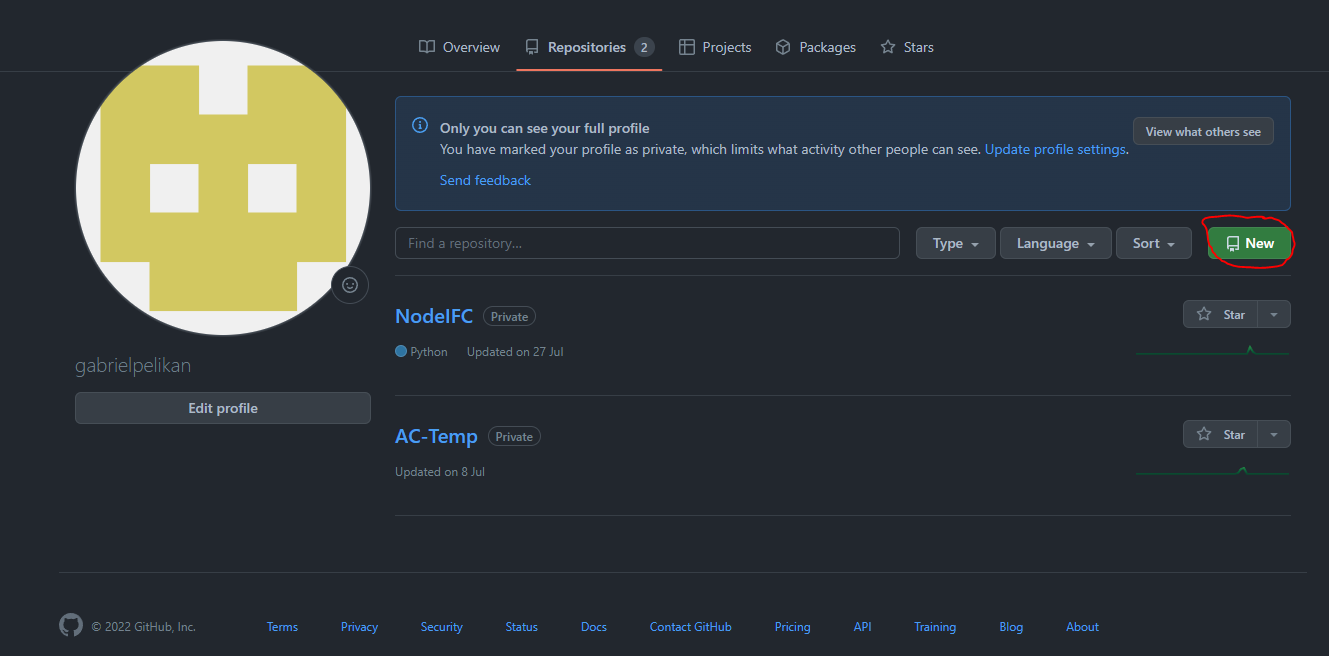
\includegraphics[width=10cm]{Neu-Repo-erstellen-1.png}
    \caption[fig:neurepo1]{Neues Repository erstellen mit \textit{New}}
\end{figure}

Nach der Eingabe einiger Informationen (Name, Sichtbarkeit, etc.) ist ein neues Repository erstellt. 

\section{Git}
\subsection{Repository initialisieren}

\begin{figure}[ht]
    \centering
    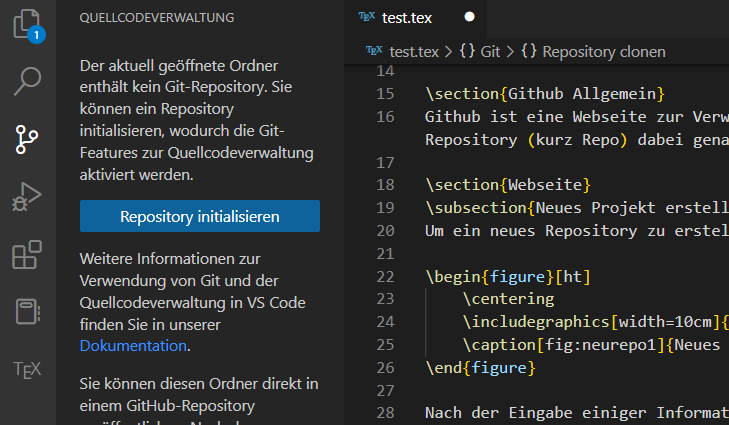
\includegraphics[width=7cm]{Repo-initialisieren.png}
    \caption[fig:repoinit1]{Repository initialisieren}
\end{figure}

\begin{figure}[ht]
    \centering
    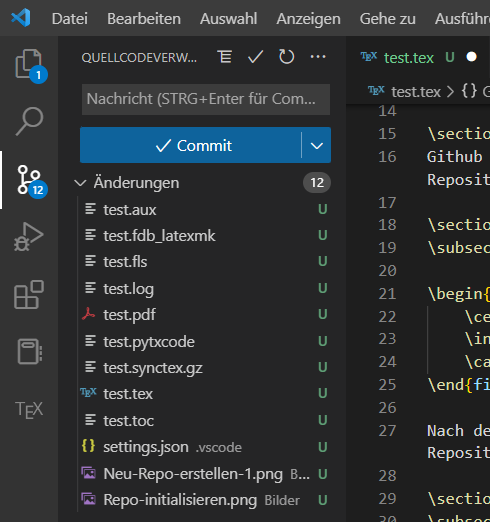
\includegraphics[width=7cm]{Repo-initalisiert.png}
    \caption[fig:repoinit2]{Repository initialisiert}
\end{figure}

\subsection{Repository commit}
Nach der Initalisierung muss man die Änderungen bereitstellen(stagen). Hierfür neben Änderungen auf das + drücken. Danach auf \textit{Commit}.

 

 

 


\end{document}